\documentclass[a4paper,12pt,titlepage]{article}
\pdfpagewidth
\paperwidth
\pdfpageheight
\paperheight



\usepackage[italian]{babel} 
\usepackage[T1]{fontenc} 
\usepackage[utf8]{inputenc} 
\usepackage{graphicx,color,listings}
\usepackage{fancyhdr} 
\usepackage{mathtools}
\usepackage{mhsetup}
\usepackage{amscd} 
\usepackage[usenames,dvipsnames]{xcolor}
\frenchspacing
\usepackage{geometry}
\usepackage{caption}
\captionsetup{labelformat=empty, textfont=sl}
\geometry{a4paper,tmargin=3cm,bmargin=3cm, lmargin=3cm,rmargin=2cm} \usepackage{multirow}

\textwidth16cm\textheight24cm\topmargin0mm\headheight0mm\headsep6mm\oddsidemargin0mm\evensidemargin0mm

\usepackage{siunitx}



\begin{document}
\author{David De Pol}
\title{Simulazione di scenari di scuotimento
sismico ad Ischia mediante l'utilizzo
della Web App XeRiS}
\maketitle
\tableofcontents
\clearpage

\section{Introduzione}

L'Italia è un'area ad elevata sismicità caratterizzata dalla presenza di numerose faglie sismicamente attive, situate nella litosfera a profondità relativamente               modeste. Si stima che nel passato esse abbiano provocato eventi 
sismici di magnitudo anche superiore a 7.0, come ad esempio il terremoto
calabro-siculo del 1908, che danneggiò gravemente le città di Reggio Calabria e Messina provocando più di novantamila morti.\\
La mappa italiana di pericolosità sismica (PCM 28 aprile 2006) segnala ampie porzioni del territorio nazionale su cui può incidere un importante fattore di rischio.

\begin{figure}[htbp]
 \centering
 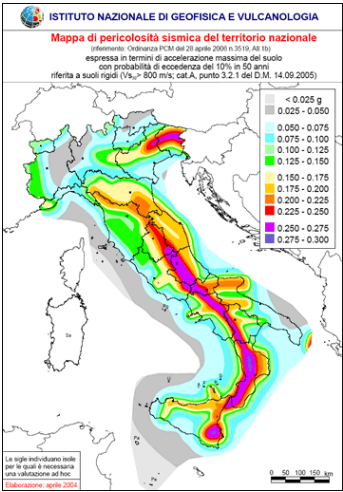
\includegraphics[width=.5\linewidth]{Img/PericolositaSismoNazionale.png}
 \caption{Mappa italiana di pericolosità sismica PCM 28 aprile 2006.}
 \label{fig:PericolositaSismoNazionale1}
\end{figure}

La pericolosità sismica è associata agli effetti fisici di un sisma che possono rivelarsi potenzialmente dannosi per l'uomo e/o le sue attività, come ad
esempio il massimo scuotimento orizzontale del suolo, solitamente espresso in PGA (Peak Ground Acceleration). Il rischio sismico, in sintesi, rappresenta
la probabilità che l'uomo, e/o le sue attività, subiscano un livello di danno se esposti a pericolosità sismica; viene valutato in concomitanza dei fattori di
pericolo, vulnerabilità ed esposizione. La vulnerabilità sismica indica la predisposizione di una costruzione a subire un determinato danno se soggetta a
un evento sismico di data entità, mentre l'esposizione descrive l'abbondanza di beni esposti al pericolo (e.g. vite umane, edifci e opere d'arte).\\
I livelli di scuotimento del suolo sono determinati principalmente dai seguenti fattori:\\

\begin{itemize}
\item  La magnitudo: indica la quantità di energia sismica rilasciata dal terremoto, ed è espressa in forma logaritmica. Tra un'unità di magnitudo e la
successiva corrispondono differenze energetiche circa di trentadue volte.
\item  La distanza epicentrale: si misura tra il sito in cui sono valutati gli effetti del sisma, e la porzione di litosfera dalla quale ha origine la rottura da cui si propagano le onde sismiche.
\item  Il processo di rottura: determina la direttività della rottura sul piano di faglia incidendo anche sulle caratteristiche del segnale sismico, percepito al sito.
\item  Le proprietà del mezzo attraversato dalle onde sismiche: gioca un ruolo fondamentale determinando i fattori di amplificazione e di decadimento
dei fronti d'onda.
\end{itemize}

Al fine di prevedere possibili scenari sismici può essere condivisibile l'idea di usare degli strumenti che permettano la simulazione di eventi sismici
realistici, basati su dati debitamente validati, misurati e/o stimati, caratterizzanti le sorgenti sismiche, i processi cinematici di rottura e gli effetti di sito.\\

In questo lavoro di tesi sono stati modellizzati eventi di scenari sismici ad Ischia, in corrispondenza della stazione sismica IOCA di Casamicciola, generati da sorgenti sismogeniche con caratteristiche tettoniche e ubicazioni geografiche differenti.\\
Gli eventi di scenario sono stati simulati utilizzando l'applicazione web XeRiS (Vaccari 2016), mentre i dati per la caratterizzazione delle sorgenti sismiche
sono stati tratti dal Database of Individual Seismogenic Sources (DISS Working Group, 2018).\\
Sono state prese in considerazione sei sorgenti sismiche: una situata sulla faglia di Casamicciola nella parte settentrionale dell'isola, le altre su alcune faglie appenniniche presenti nell'Italia meridionale, a una distanza di circa cento chilometri dal sito scelto.\\
Per quanto riguarda l'attribuzione delle caratteristiche geo-sismologiche utilizzate nella simulazione in cui la sorgente è posizionata sulla faglia di
Casamicciola, si è deciso di utilizzare quelle concernenti il terremoto di Casamicciola del 21 agosto 2017 (M=4), rilevate alla stazione sismica IOCA e
stimate da sismologi e geofisici. Tale decisione consegue dal fatto che è necessario mantenere sotto controllo il grado di consistenza tra le previsioni
ottenute e gli eventi sismici realmente accaduti. Non si avrà la pretesa di ottenere come risultato delle simulazioni dei livelli di scuotimento del suolo coincidenti a quelli effettivamente rilevati, ma una stima ragionevole di quanto ci si può attendere in futuro per eventi simili.\\
Si è deciso di simulare questo terremoto specifico poiché presenta delle caratteristiche particolari (e.g. De Natale, 2018), che possono essere approfondite al fine di dare un contributo alla stesura di nuove mappe di pericolosità per l'Isola d'Ischia più realistiche rispetto a quelle adottate dalla normativa nazionale attuale.\\
Il lavoro svolto è costituito di tre parti: nella prima sono presentate le funzionalità utilizzate dell'applicazione web XeRiS, e riportati i dati geosismologici relativi alla sorgete sismica di Casamicciola. Nella seconda parte sono presentati i risultati della simulazione con sorgente sull'isola, tabulate le faglie appenniniche e presentati i relativi scenari di scuotimento ad Ischia. Nella terza e ultima parte sono confrontati i diversi scenari di scuotimento simulati.

\section{Presentazione della Web App XeRiS}

XeRiS è un'applicazione web (in inglese Web App) (Vaccari, 2016), che permette la valutazione neo-deterministica della pericolosità sismica (Panza et al., 2001, Panza et al., 2012) mediante un'intuitiva interfaccia utente, nascondendo all'utente finale le complessità insite nel motore di calcolo.\\
Attraverso la simulazione di eventi sismici e il calcolo di scenari di scuotimento realistici, valutati in un singolo sito d'interesse o in un'area attorno all'epicentro, si possono calcolare i parametri di scuotimento del suolo, come ad esempio la Peak Ground Acceleration (PGA), tipicamente adottata per la stima della pericolosità sismica. Ma XeRiS genera anche le serie temporali, in spostamento, velocità ed accelerazione, che possono essere utilizzate dagli ingegneri come input sismico per la progettazione di strutture resistenti al sisma.\\
Con valutazione neo-deterministica della pericolosità, si intende che per la costruzione degli scenari di scuotimento sismico, si tengono in considerazione il modello della sorgente, le modalità di propagazione del segnale e gli effetti di sito, rispettando le leggi fisiche che descrivono la generazione e la propagazione delle onde sismiche.
\begin{figure}[htbp]
 \centering
 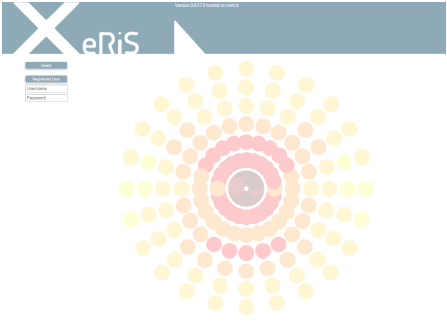
\includegraphics[width=.5\linewidth]{Img/XerisLogIn.png}
 \caption{Login XeRiS}
 \label{fig:Login XeRiS2}
\end{figure}
Inizialmente XeRiS richiede la definizione di un modello strutturale stratificato per la porzione di litosfera, nella quale noi collocheremo la faglia, in cui ha origine il processo di rottura e da cui si propagheranno i fronti d'onda del sisma. E' possibile selezionarne uno già implementato oppure utilizzarne di nuovi creati ad hoc.\\
Successivamente, si modellizza la sorgente sismica attribuendone le caratteristiche geo-sismologiche, nel nostro caso quelle disponibili nel Database of Individual Seismogenic Sources (DISS Working Group, 2018).\\
Per rappresentare al meglio la fisica del problema, la sorgente sarà considerata estesa, e dunque non trattata come un punto materiale posizionato in corrispondenza dell'ipocentro del terremoto, bensì approssimata ad una superficie rettangolare di dimensioni appropriate (e.g. Wells and Coppersmith, 1994), contenente al suo interno delle sotto-sorgenti che potranno essere considerate puntiformi.\\
Dopo aver scelto il sito d'interesse, nel caso in esame le coordinate della stazione sismica IOCA di Casamicciola sull'Isola d'Ischia, avrà luogo il calcolo dei segnali sismici che potranno essere utilizzati come input sismico.\\
In questo modo sarà generata una banca dati per un insieme di terremoti di scenario con caratteristiche tettoniche e ubicazioni geografiche differenti, utile per confrontare gli effetti ad Ischia dei diversi terremoti e quindi anche al fine di valutare quale evento sismico possa determinare una maggior pericolosità.
\clearpage

\subsection{Definizione del modello strutturale}


\subsection{Modellizzazione di sorgenti sismiche estese}
\subsection{Modellazione del moto del suolo generato da sorgenti sismiche
estese}
\subsection{Parametri di scuotimento del suolo}
\subsection{Test parametrici}

\section{Simulazione di eventi di scenario}
\subsection{Simulazione del terremoto a Ischia: Faglia di Casamicciola}
\subsection{ Simulazione di eventi di scenario ad Ischia per sorgenti appenniniche}
\subsection{Confronto tra alcune simulazioni con sorgente appenninica}

\section*{Conclusioni}\addcontentsline{toc}{section}{Conclusioni}

\end{document}